\documentclass[11pt,a4paper]{article}
\usepackage{fontspec}
\usepackage[english]{babel}
\usepackage[margin=2.1cm]{geometry}
\usepackage{booktabs,array,tabularx}
\usepackage{xcolor}
\usepackage{graphicx}
\usepackage{pgfplots}
\pgfplotsset{compat=1.17}
\PassOptionsToPackage{hyphens}{url}
\usepackage[hidelinks]{hyperref}
\usepackage{enumitem}
\setlist{nosep,leftmargin=1.4em}
\emergencystretch=3em

\definecolor{impl}{HTML}{3B6EA8}
\definecolor{rev}{HTML}{8FB3DA}

\title{Sweatshop on P-Chess: the UI redo's profile and repertoire screens\\\large Profile (UI-027), repertoires, opening picker and editor (UI-028) and visible field labels (UI-029); GPT-6.1 Terra lineup, lane \texttt{ui-screens}}
\author{Foreman, session \texttt{sweatshop/ui-screens/2026-10-31-1731}}
\date{31 October 2026}

\begin{document}
\maketitle

\section*{Summary}

First run of the \texttt{ui-screens} lane, in its clone at \path{.artifacts-build/lanes/ui-screens},
side by side with the \texttt{ui-game} and \texttt{ui-review} lanes. UI-021 (the shared theme) was
already on \texttt{main}. Four driver launches (17:30, 18:24, 19:16, 20:00), last merge at 20:13,
session PR \href{https://github.com/Laginho/P-Chess/pull/34}{\#34}.

\begin{itemize}
  \item \textbf{Produced:} the three lane tickets merged on the session with
        \texttt{Verdict: Approve}: UI-027, UI-028 and UI-029, all \texttt{Review: agent}. CLEAN-012
        (shared font weights) is recorded \texttt{done} as superseded by the owner's PR \#37; this
        lane's own attempt at it was stopped before review. Sync gate on the session with
        \texttt{main}: 436 passed, 0 failed (6 Lc0 skips).
  \item \textbf{Cost:} \textbf{\$13.62} at API list price over 15 stages, all priced:
        \texttt{gpt-6.1-terra xhigh} implementing \$6.95 (9), \texttt{gpt-6.1-sol xhigh} reviewing
        \$6.67 (6). Codex quota: 10 points of the weekly window (Terra xhigh 4, Sol xhigh 5,
        1 outside the stages; $\pm$1 per stage, the total is exact), no reset. Two sibling lanes ran
        on the same account at the same time.
  \item \textbf{What went wrong:} the shared font-weight defect from UI-021 blocked UI-027 and was
        filed three times across the lanes (UI-030, CLEAN-012 twice); the owner fixed it on
        \texttt{main} while this lane was implementing its own copy. Terra xhigh twice ended a
        UI-028 session early at a checkpoint. Three driver/ticket-flow defects each parked or
        corrupted one handoff (Driver and runtime issues).
  \item \textbf{Provisional verdict:} code quality was good (every fix test-first, 5 real
        findings, no noise), but the lane needed eight foreman interventions to finish. Terra xhigh
        is not immune to early stops on a three-screen ticket.
\end{itemize}

\section*{What was done}

\textbf{UI-027}: the Profile follows \texttt{Profile.png}: a name card with the initial avatar,
``Playing since'' from the first saved game and the Name field with Save; four tiles (Games,
Avg.\ accuracy, W/D/L in green, grey and red, Flag W/L); the results table per level and time
control with flag wins and losses summed per level; the accuracy chart over every analysed game.
\path{docs/spec.md} §15.8 says so. Main files \path{ui/profile.gd}, \path{ui/profile.tscn},
\path{ui/accuracy_chart.gd}. Reopened once: with a full history the table and tiles did not match
the design (11~px cells, centred Level, no dividers or flag colours, 8~px tile padding); stage 2
had only compared a one-row fixture. Then blocked once on the shared font weights, which
\path{ui/theme/p_chess.tres} declared with string \texttt{"wght"} keys that Godot 4.7 ignores.

\textbf{UI-028}: Repertoires shows the repertoires as cards (colour dot, name, line count and
origin, a pencil that opens the editor), the selected repertoire's lines, and the board with
$\leftarrow$/$\rightarrow$ and the line's moves; the From openings picker is a modal with Name,
White/Black, a tree with partial checkboxes and Create repertoire; the editor shows the board and a
card with ``Unsaved changes'', a compact numbered move tree, a trash button per branch, Cancel and
Save. Repertoire files now remember their origin (an optional \texttt{source} key, a proxy
decision). Main files \path{ui/repertoire_screen.gd}, \path{ui/opening_picker.gd},
\path{ui/repertoire_editor.gd}, \path{bot/repertoire.gd}. Reopened once: a 99-character name
pushed the board and Save off-screen at 800$\times$600 (the headings had no width bound), and a
line starting with Black was numbered \texttt{1.e5 e4} (\path{ui/repertoire_screen.gd} counted by
array parity).

\textbf{UI-029}: the import and opening-picker text fields keep a visible label after you type,
instead of a placeholder that disappears. Main files \path{ui/repertoire_import.tscn},
\path{ui/opening_picker.tscn}. Not reopened. Its first approval was void: stage 2 reviewed and
merged its own work; an independent review later approved it.

\section*{Timeline}

{\small
\begin{tabularx}{\linewidth}{@{}lX@{}}
\toprule
17:30 & Clone made from \texttt{acb4662}, assets imported; launch 1, default lineup (Terra). \\
17:39--17:45 & UI-027 to review (7~min), reopened (table and tiles; UI-030 filed for fonts). \\
17:52--18:06 & UI-027 fixed (7~min); review blocks it on UI-030, proxy escalates. \\
18:13--18:19 & UI-028 stops early twice (6~min each, real progress); parked, run 1 ends. \\
18:22--18:24 & Foreman asks the proxy: relaunch from the branch. Launch 2. \\
19:02--19:09 & UI-028 to review (37~min), reopened (long names, Black-start numbers; CLEAN-012 filed). \\
19:15--19:16 & UI-028 fixed (6~min), parked on a stale gate line; foreman relabels it. Launch 3. \\
19:32 & UI-028 merged; fonts deferred by the proxy; CLEAN-012 moved into this lane. \\
19:43--19:45 & UI-029 handed off on a branch the driver cannot see; attempt 2 self-reviews and merges. \\
19:51--19:52 & Owner merges CLEAN-012 to \texttt{main} (PR \#37); STOP after this lane's duplicate attempt. \\
19:58--20:00 & Sync with \texttt{main} (gate 436/0); UI-027 and UI-029 back to review. Launch 4. \\
20:09--20:13 & UI-027 and UI-029 merged by independent reviews. Nothing left. \\
\bottomrule
\end{tabularx}
}

\section*{Per stage}

{\small
\begin{tabularx}{\linewidth}{@{}llllrrrrrX@{}}
\toprule
When & Ticket & Stage & Model & Min & In & Cache & Out & Cost & Outcome \\
\midrule
17:39 & UI-027 & impl & terra xhigh & 7 & 5.3M & 98\% & 15k & 0.42 & to-review \\
17:45 & UI-027 & review & sol xhigh & 6 & 3.7M & 95\% & 20k & 0.94 & reopened \\
17:52 & UI-027 & impl & terra xhigh & 7 & 5.3M & 98\% & 14k & 0.41 & to-review \\
18:06 & UI-027 & review & sol xhigh & 15 & 6.1M & 97\% & 24k & 1.22 & blocked \\
18:13 & UI-028 & impl & terra xhigh & 6 & 5.0M & 98\% & 17k & 0.41 & failed \\
18:19 & UI-028 & impl & terra xhigh & 6 & 5.2M & 98\% & 17k & 0.43 & failed \\
19:02 & UI-028 & impl & terra xhigh & 37 & 64.4M & 100\% & 80k & 3.80 & to-review \\
19:09 & UI-028 & review & sol xhigh & 6 & 5.4M & 96\% & 25k & 1.15 & reopened \\
19:15 & UI-028 & impl & terra xhigh & 6 & 5.1M & 99\% & 9k & 0.37 & parked \\
19:32 & UI-028 & review & sol xhigh & 15 & 6.1M & 95\% & 30k & 1.44 & merged \\
19:43 & UI-029 & impl & terra xhigh & 11 & 6.0M & 99\% & 11k & 0.42 & failed$^a$ \\
19:45 & UI-029 & impl & terra xhigh & 2 & 2.4M & 95\% & 8k & 0.28 & failed$^b$ \\
19:51 & CLEAN-012 & impl & terra xhigh & 6 & 4.8M & 97\% & 9k & 0.41 & to-review$^c$ \\
20:09 & UI-027 & review & sol xhigh & 8 & 5.3M & 96\% & 22k & 1.14 & merged \\
20:13 & UI-029 & review & sol xhigh & 4 & 3.1M & 94\% & 14k & 0.78 & merged \\
\midrule
 & & & & 142 & 133.2M & & 315k & 13.62 & \\
\bottomrule
\end{tabularx}
}

{\footnotesize $^a$ The row lies: the stage reached \texttt{to-review}, on a branch the driver could
not find. $^b$ The row lies the other way: the stage reviewed and merged its own work.
$^c$ Duplicate of PR \#37, never reviewed.\par}

\begin{center}
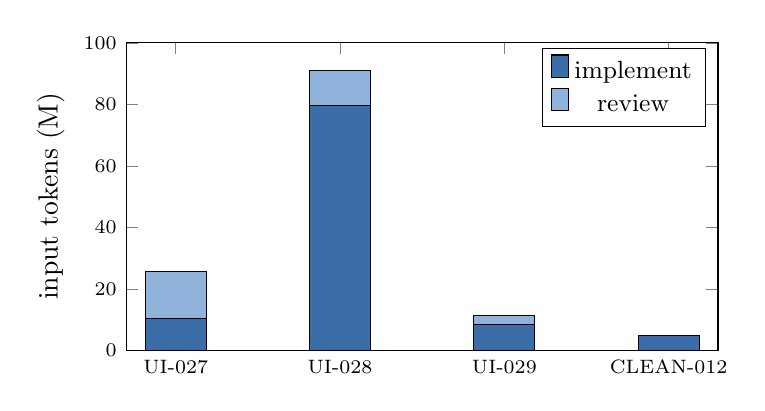
\begin{tikzpicture}
\begin{axis}[ybar stacked, bar width=22pt, width=0.75\linewidth, height=5.5cm,
  symbolic x coords={UI-027,UI-028,UI-029,CLEAN-012},
  xtick=data, ylabel={input tokens (M)}, ymin=0, legend style={at={(0.98,0.98)},anchor=north east,font=\small},
  tick label style={font=\scriptsize}]
\addplot[fill=impl] coordinates {(UI-027,10.6) (UI-028,79.7) (UI-029,8.4) (CLEAN-012,4.8)};
\addplot[fill=rev] coordinates {(UI-027,15.1) (UI-028,11.5) (UI-029,3.1) (CLEAN-012,0)};
\legend{implement, review}
\end{axis}
\end{tikzpicture}
\end{center}

Wasted: CLEAN-012's duplicate (\$0.41) and UI-029's self-review (\$0.28), \$0.69 or 5\% of the run.
UI-028's two early stops (\$0.83) kept their 15 commits, which the third attempt resumed. UI-027's
blocked review (\$1.22) was the price of a prerequisite outside the lane. Input is 78\%
implementation, 48\% in UI-028's single 37-minute stage.

\section*{Comparison with previous runs}

From \texttt{run-log.md}. The sibling \texttt{ui-game} lane: \$9.03 for 3 merged tickets (\$3.01
each), every ticket reopened once, no failed stage. This run: \$13.62 for 3 (\$4.54 each), two
reopened, five stages that did not reach review. UI-028's first complete implementation (37~min,
\$3.80) is the most expensive Terra stage so far; the \texttt{ui-game} lane's longest was 27~min.
Reviews cost \$0.78--1.44 (\$0.46--1.10 there).

\section*{Observations per model}

\begin{itemize}
  \item \textbf{gpt-6.1-terra xhigh, stage 2} (9 stages, 4 tickets): every fix test-first with
        the red run recorded. It ended UI-028's first two sessions on its own at about 6~min with a
        progress report, on a three-screen ticket; the third, after a foreman note ``do not end the
        session at a checkpoint'', ran 37~min to a full handoff. It handed UI-027 off with a
        one-row fixture and asked the reviewer to do the populated comparison. On UI-029 it found
        its own branch at \texttt{to-review} and ran stage 3 on itself.
  \item \textbf{gpt-6.1-sol xhigh, review} (6 stages, 4--15~min): every finding was reproduced
        with a probe and numbers (rects at 800$\times$600, a Black-start PGN, TextServer
        coordinates). It refused to work around the shared font defect inside the screens, which
        was right, but filed it twice in the \texttt{ui-base} folder, where no driver runs. Its
        UI-029 review used the foreman's review range correctly.
  \item \textbf{opus-5.5 xhigh, proxy}: five calls. It escalated UI-027's font prerequisite and,
        an hour later, deferred the same defect for UI-028 as a release condition. Both were
        defensible; together they are inconsistent.
\end{itemize}

\section*{Driver and runtime issues}

\begin{enumerate}
  \item \textbf{First \texttt{Gate evidence:} line wins.} \texttt{GateEvidenceField} in
        \path{driver.ps1} takes the first match. UI-028's fix appended a new receipt below the old
        one, so a valid handoff (receipt for \texttt{42fa431}, equal to production) was parked as
        ``code changed after gate''.
  \item \textbf{Case-sensitive branch discovery.} \texttt{Find-TicketBranch} matches
        \texttt{UI-029} case-sensitively, and \texttt{ui-029} only exactly. Stage 2 named its branch
        \texttt{ui-029-visible-field-labels}; the driver logged a completed handoff as failed.
  \item \textbf{Stage 2 can run stage 3.} The retry was sent the bare id, found the branch at
        \texttt{to-review} and, as \texttt{ticket-flow} dispatches by Stage, reviewed and merged its
        own work on the session. The driver then marked the ticket blocked on top of the merge.
  \item Codex rejected one inline PowerShell \texttt{-Command} by policy in UI-027's first stage;
        the stage went on.
  \item A T3 server restart killed the foreman's watch loops at 17:53; the detached driver was
        unaffected. Shutdown 1.0--1.6~s per stage; no crash, timeout or API error.
  \item The new clone needed \texttt{godot --headless --import} and
        \texttt{*.uid}/\texttt{*.import} in \path{.git/info/exclude}; the import rewrote
        \path{fonts/NotoSans-Variable.ttf.import} line endings (restored by checkout).
\end{enumerate}

\section*{Recommendations}

\begin{enumerate}
  \item Make the driver read the \emph{last} \texttt{Gate evidence:} line, or have stage 2 replace
        it on a reopen (issue 1).
  \item Make \texttt{Find-TicketBranch}'s pattern case-insensitive (issue 2).
  \item When the driver retries stage 2 and the branch already reads \texttt{to-review}, start
        stage 3 on the reviewer's model instead of sending the bare id to the implementer
        (issue 3).
  \item When a review files a ticket outside its own lane, say so in the driver's \texttt{.out}
        and the PR body: UI-030 and CLEAN-012 landed in \path{.scratch/ui-base/issues/}, where no
        driver ran, and three lanes filed the same defect (both copies took prefix \texttt{82}).
  \item Terra xhigh: split three-screen tickets, or state in the ticket that the session ends only
        at \texttt{to-review}. Scoreboard rows: \texttt{gpt-6.1-terra xhigh} 18 $\to$ 27 stage
        runs, 0 $\to$ 5 failed (4 of the 5 were early stops or driver misreads in this run).
\end{enumerate}

\section*{Human debt and proxy decisions}

No \texttt{Débito humano:} lines in this run's tickets. Proxy calls, all by
\texttt{opus-5.5 xhigh} (Codex reached the proxy directly):

\begin{itemize}
  \item UI-028 (stage 2): \texttt{Proxy decided}: ``Add the seam: an optional \texttt{"source"}
        key in the existing version-1 file, persisted for new saves and carried through edits. A
        legacy file without the key shows only `N lines', with no origin suffix.''
  \item UI-027 (stage 3): \texttt{Proxy escalated}: ``UI-027 can't pass criterion 6 or be merged
        until UI-030 lands, and UI-030 can't run from this lane. [\ldots] Someone has to push to
        main and start a lane, and that's the owner's or parent's call.'' Resolved by the owner's
        PR \#37.
  \item UI-028 (foreman): \texttt{Proxy decided}: ``Relaunch the lane so stage 2 picks up branch
        \texttt{ui-028} again for two more attempts. Leave splitting for later.'' It recommended
        \texttt{-Lineup sol}; the run kept the default Terra lineup the parent asked for.
  \item UI-028 (stage 3): \texttt{Proxy decided}: ``Accept a release-level deferral of the shared
        font weights to CLEAN-012, so UI-028 can merge into the session once the Spec re-review is
        clean.''
  \item UI-029 (stage 2): \texttt{Proxy decided}: ``Yes. Stage 2 may test real instantiated scenes
        for visible labels, but the screenshots go in Verification as manual evidence, not in the
        tests.''
\end{itemize}

\section*{Acceptance}

Probes on the session after the sync with \texttt{main} (\texttt{9ad4daf}): the headless gate (436
passed, 0 failed, 6 Lc0 skips); the final UI-027 review's fresh gate and populated Profile
captures with the real weights; UI-029's six corrected-font captures. The foreman captured Profile,
Repertoire, OpeningPicker, RepertoireEditor and RepertoireImport at 1280$\times$800 and
800$\times$600 with \path{scripts/screens.gd}, at the lane base \texttt{acb4662} (before) and the
session head (after), in \path{%TEMP%/pchess-ui-screens-shots/}. Seen in them: the weights now
render; at 800$\times$600 the app-wide Settings button shows above the editor modal's top edge
(observed, not judged). Not examined: physical input, the full opening catalog, live Lc0, the
99-character name after the font fix, and Bruno's visual comparison.

\section*{Reopen attribution}

Labelled by the foreman (opus-5.5); the reviewer was \texttt{gpt-6.1-sol xhigh}, so no
self-judging. Rows appended to \path{.scratch/reopen-attribution.md}.

{\small\noindent
\begin{tabularx}{\linewidth}{@{}>{\raggedright\arraybackslash}p{1.7cm}X>{\raggedright\arraybackslash}p{2.7cm}X@{}}
\toprule
Ticket (round) & Finding & Label & Why \\
\midrule
UI-027 (1) & Table and tiles differ from the design with a full history & S2-explícito/\allowbreak código & criterion 6; stage 2 checked only a one-row fixture \\
UI-027 (1) & Shared font weights render at 400 & S1 ? & UI-021's defect, outside Primary files; needed a scope decision. Review miss: UI-021 \\
UI-028 (1) & Long name pushes board and Save off-screen at 800$\times$600 & S2-explícito/\allowbreak código & criterion 4 carries shared acceptance 2 \\
UI-028 (1) & Black-start line numbered by array parity & S2-implícito & its own editor already numbered from the start side \\
UI-028 (1) & Shared font weights render at 400 & S1 ? & same UI-021 defect; deferred, then fixed by PR \#37 \\
\bottomrule
\end{tabularx}
}

Totals, reopens: S2-explícito/código 2, S2-implícito 1, S1 2 (both borderline, both the same
UI-021 defect), S3-ruído 0; fixed in review: none. No review-induced churn, no drip-feed. The font
defect's post-approval row (\texttt{session-review}, UI-021, review miss \texttt{yes}) was already
recorded by the \texttt{ui-game} lane and is not counted again.

\section*{Scoreboard}

\texttt{scoreboard.ps1} over the ClassyCall, EasyMath, PhysiSyst, SIGAA-ME and SynchroNice main
checkouts plus this lane's clone in place of P-Chess's main checkout (same merged run log; it holds
this run's attribution rows). Moved since the \texttt{ui-game} report: implementer
\texttt{gpt-6.1-terra xhigh} 18 $\to$ 27 stage runs, 0 $\to$ 5 failed; pair
\texttt{gpt-6.1-terra xhigh} $\rightarrow$ \texttt{gpt-6.1-sol xhigh} 17 $\to$ 20 reviews, 35\% $\to$
40\% reopened (S2 rate 40\%); the same reviewer over \texttt{gpt-6.1-terra high} stays at 30\% (20)
and over \texttt{gpt-6.1-sol high} at 23\% (22). With 20 reviews, Terra xhigh now trails both under
the same reviewer. Interventions: human-rescue 30 $\to$ 31, automatic-recovery 110 $\to$ 112,
proxy-decision (opus-5.5 xhigh) 11 $\to$ 15.

{\tiny
\begin{verbatim}
| Implementer | Stage runs | To review | Failed | Asked | Median min to review | Cost |
|---|---|---|---|---|---|---|
| gpt-6.1-sol high | 68 | 63 | 0 | 5 | 9m | $47.66 (68/68 priced) |
| opus-5.5 xhigh | 18 | 14 | 4 | 0 | 12m | $91.78 (18/18 priced) |
| gpt-6.1-sol max | 6 | 5 | 0 | 1 | 24m | $12.12 (6/6 priced) |
| opus-5.5 high | 20 | 13 | 6 | 1 | 6m | $37.46 (20/20 priced) |
| gpt-6.1-sol xhigh | 10 | 10 | 0 | 0 | 12m | $7.57 (10/10 priced) |
| gpt-6.1-terra high | 32 | 20 | 10 | 2 | 7m | $8.54 (32/32 priced) |
| gpt-6.1-terra xhigh | 27 | 21 | 5 | 1 | 9m | $18.02 (27/27 priced) |
(rows for older models unchanged since the ui-game report)

| Implementer | Reviewer | Reviews | Reopened | Reopen rate | Reopened for S2 | S2 rate | Unclassified | Fixed in review for S2 |
|---|---|---|---|---|---|---|---|---|
| gpt-6.1-sol high | gpt-6.1-sol max | 38 | 12 | 32% | 9 | >=24% | 2 | 1 |
| gpt-6.1-sol high | gpt-6.1-sol xhigh | 22 | 5 | 23% | 5 | 23% | 0 | 0 |
| gpt-6.1-sol xhigh | gpt-6.1-sol xhigh | 10 | 1 | 10% | 1 | 10% | 0 | 1 |
| gpt-6.1-terra high | gpt-6.1-sol xhigh | 20 | 6 | 30% | 6 | 30% | 0 | 0 |
| ? | gpt-6.1-sol xhigh | 4 | 1 | 25% | 0 | 0% | 0 | 0 |
| gpt-6.1-terra xhigh | gpt-6.1-sol xhigh | 20 | 8 | 40% | 8 | 40% | 0 | 2 |
(other pairs unchanged since the ui-game report)

| Implementer -> Reviewer | Rounds | S2 explicit code | S2 explicit test | S2 implicit | S1 | S3 noise |
|---|---|---|---|---|---|---|
| gpt-6.1-terra high -> gpt-6.1-sol xhigh | 9 | 10 | 1 | 3 | 1 | 0 |
| gpt-6.1-terra xhigh -> gpt-6.1-sol xhigh | 10 | 9 | 0 | 6 | 2 | 0 |

| Discovery | Recorded findings | Earlier review miss (yes / known) | Review-induced churn (yes / known) |
|---|---|---|---|
| ticket-review | 397 | 7 / 202 | 1 / 204 |
| session-review | 32 | 25 / 27 | 0 / 31 |
| release-audit | 2 | 2 / 2 | 0 / 2 |
Runtime completion to process exit: 361.531s total over 287 measured stages; 334 unmeasured.
| Intervention | Recorded events |
|---|---|
| human-rescue | 31 |
| automatic-recovery | 112 |
| proxy-decision (unknown) | 37 |
| routine-approval | 18 |
| proxy-decision (gpt-6-astra high, fallback) | 58 |
| proxy-decision (opus) | 42 |
| proxy-decision (supervisor) | 12 |
| proxy-decision (opus-5.5 xhigh) | 15 |
\end{verbatim}
}

The UI-029 review is charged to \texttt{?} (row \texttt{? $\rightarrow$ gpt-6.1-sol xhigh}, 2
$\to$ 4): its last hand-off to review was the foreman's.

\section*{Pending for the human}

\begin{enumerate}
  \item Review and merge PR \#34 (three tickets, all \texttt{Review: agent}); it is synced with
        \texttt{main} at \texttt{0635b3d}. After it merges, tell the other open lanes to sync.
  \item Compare \path{%TEMP%/pchess-ui-screens-shots/after/} with the references; check the
        Settings button over the editor modal at 800$\times$600.
  \item By hand: create a repertoire from openings, open it with the pencil, add and delete a
        branch, save; rename yourself on Profile; type in the import and picker fields.
\end{enumerate}

\end{document}
